\documentclass[tikz]{standalone}
\usepackage{pgfplots}
\begin{document}

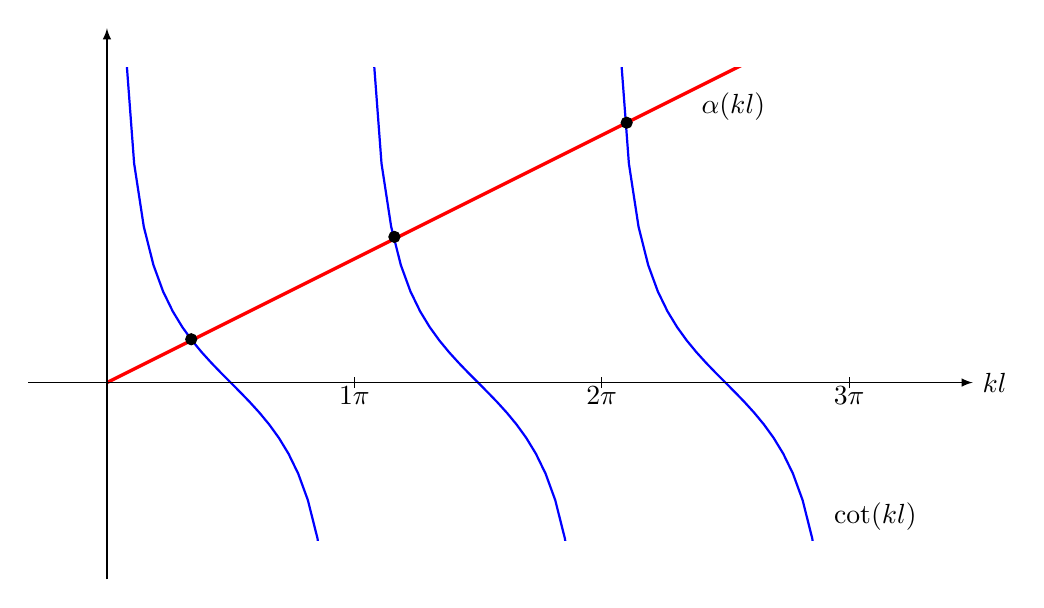
\begin{tikzpicture}[>=latex]

    \begin{scope}
        % On trace 3 périodes de cotan
        \clip (-1,-2) rectangle (3.5*pi,4);
        \foreach \i in {1,2,3} {
            \def\start{0.1+(\i-1)*pi}
            \def\stop{\i*pi-0.1}
            \draw [blue, thick, domain=\start:\stop] plot(\x,{cot(\x r)});
        }
        \draw [domain=0:3.2*pi, red, very thick] plot(\x,.5*\x);
        \draw (2.7*pi,3.5) node[left] {$\alpha(kl)$};
        \draw (2.9*pi,-1.7) node[right] {$\mathrm{cot}(kl)$};
    \end{scope}
    % \draw [step=.2] (-5,-5) grid (10,10);
    % \draw [red, thick] (-5,-5) grid (10,10);
    % axes
    \draw[->] (-1,0) -- (3.5*pi,0) node[right] {$kl$}; % x
    \draw[->] (0,-2.5) -- (0,4.5); % y
    \foreach \i in {1,2,3} \draw (\i*pi,-2pt) -- (\i*pi,2pt) node [below] {$\i\pi$};
    \foreach \x/\y in {1.07/.55,3.65/1.85,6.6/3.3} {
        \draw[fill=black] (\x,\y) circle (2pt);
    }
\end{tikzpicture}

\end{document}
